\documentclass[12pt,a4paper]{article}
% ============================================================
%  Оформление отчёта. Обычно здесь ничего менять не нужно.
%  Сборка по умолчанию выполняется XeLaTeX.
% ============================================================

\usepackage{iftex}
\ifPDFTeX
  \usepackage[T2A]{fontenc}
  \usepackage[utf8]{inputenc}
\else
  \usepackage{fontspec}
  \setmainfont{Liberation Serif}
  \setmonofont{Liberation Mono}[Scale=MatchLowercase]
\fi
\usepackage[english,russian]{babel}

% --- Поля и абзацы (как в исходном doc-шаблоне курса) ---
\usepackage[a4paper, margin=2.54cm]{geometry}
\setlength{\parindent}{0pt}
\setlength{\parskip}{4pt plus 1pt}
\frenchspacing

% --- Заголовки разделов без номеров ---
\usepackage{titlesec}
\setcounter{secnumdepth}{0}
\titleformat{\section}{\large\bfseries}{}{0pt}{}
\titleformat{\subsection}{\normalsize\bfseries}{}{0pt}{}
\titlespacing*{\section}{0pt}{14pt plus 4pt minus 2pt}{4pt plus 2pt}
\titlespacing*{\subsection}{0pt}{10pt plus 2pt minus 2pt}{3pt plus 1pt}

% --- Таблицы, рисунки, подписи ---
\usepackage[table]{xcolor}
\usepackage{graphicx}
\usepackage{tabularx}
\usepackage{float}
\usepackage{caption}
\DeclareCaptionLabelSeparator{spacedendash}{~-- }
\captionsetup{labelsep=spacedendash, font=small, singlelinecheck=false, justification=raggedright}
\captionsetup[table]{position=top, skip=4pt}
\DeclareCaptionType[fileext=lol]{listing}[Листинг][Листинги]
\captionsetup[listing]{position=top, skip=4pt, hypcap=false}
\addto\captionsrussian{%
  \renewcommand{\figurename}{Рисунок}%
  \renewcommand{\tablename}{Таблица}%
}
\newcommand{\thead}[1]{\multicolumn{1}{|c|}{\cellcolor{gray!20}\textbf{#1}}}
% Колонки таблиц без растягивания пробелов: L – резиновая, P{ширина} – фиксированная
\newcolumntype{L}{>{\raggedright\arraybackslash}X}
\newcolumntype{P}[1]{>{\raggedright\arraybackslash}p{#1}}

% --- Код и вывод терминала ---
% code     – фрагмент исходного кода;
% terminal – вывод программы, strace и т. п.;
% \inputterminal{файл} / \inputcode{файл} – то же, но из файла.
\usepackage{fvextra}
\fvset{breaklines=true, breakanywhere=true,
       frame=leftline, framerule=1.5pt, framesep=6pt,
       rulecolor=\color{gray!60}, xleftmargin=4pt}
\DefineVerbatimEnvironment{code}{Verbatim}{fontsize=\small}
\DefineVerbatimEnvironment{terminal}{Verbatim}{fontsize=\footnotesize}
\newcommand{\inputcode}[2][]{\VerbatimInput[fontsize=\small,#1]{#2}}
\newcommand{\inputterminal}[2][]{\VerbatimInput[fontsize=\footnotesize,#1]{#2}}
% Листинг с подписью сверху:
%   \begin{listingblock}{Подпись} \begin{code}...\end{code} \end{listingblock}
\newenvironment{listingblock}[1]
  {\par\medskip\captionof{listing}{#1}\nopagebreak\vspace{-\topsep}\vspace{-\parskip}}
  {\par}

% Приложение: с новой страницы, заголовок «Приложение А. ...»,
% листинги внутри нумеруются А.1, А.2, ...
\newcounter{appendixno}
\newcommand{\appendixsection}[2]{%
  \clearpage
  \section{Приложение #1. #2}%
  \stepcounter{appendixno}%
  \setcounter{listing}{0}%
  \renewcommand{\thelisting}{#1.\arabic{listing}}%
  \renewcommand{\theHlisting}{app\arabic{appendixno}.\arabic{listing}}}

% --- Ссылки ---
\usepackage[hidelinks]{hyperref}
\usepackage{xurl}

% --- Подсказки шаблона: серый курсив, удалить перед сдачей ---
\newcommand{\hint}[1]{\leavevmode{\color{gray}\itshape #1}}
% Рамка-заглушка вместо рисунка
\newcommand{\placeholder}[2][4.5cm]{%
  \fbox{\parbox[c][#1][c]{0.95\linewidth}{\centering\hint{#2}}}}

\usepackage{amsmath}
\newcommand{\ReportLab}{3}
\newcommand{\ReportStudent}{В. Е. Авраменко}
\newcommand{\ReportGroup}{М8О-204БВ-25}
\newcommand{\ReportTeacher}{Н. А. Гапонов}
\newcommand{\ReportDate}{20.10.2026}
\newcommand{\ReportYear}{2026}
\newcommand{\ReportCourse}{Операционные системы и архитектура компьютера}
\begin{document}
\setlength{\emergencystretch}{3em}
% Титульный лист
\begin{titlepage}
  \centering\large

  МОСКОВСКИЙ АВИАЦИОННЫЙ ИНСТИТУТ\\
  (НАЦИОНАЛЬНЫЙ ИССЛЕДОВАТЕЛЬСКИЙ УНИВЕРСИТЕТ)\par
  \vspace{18pt}
  Институт №8 «Компьютерные науки и прикладная математика»\\
  Кафедра 806 «Вычислительная математика и программирование»\par

  \vspace{\stretch{1.2}}

  {\bfseries Отчёт по лабораторной работе №3\\
  по курсу «\ReportCourse»\par}

  \vspace{\stretch{1.6}}

  \begin{flushright}
    \begin{tabular}{r@{\hspace{0.6em}}l}
      Выполнил:      & \ReportStudent \\[2pt]
      Группа:        & \ReportGroup   \\[2pt]
      Преподаватель: & \ReportTeacher \\[2pt]
      Дата:          & \ReportDate    \\[2pt]
      Оценка:        & \rule[-2pt]{4.2cm}{0.4pt} \\
    \end{tabular}
  \end{flushright}

  \vspace{\stretch{1}}

  Москва, \ReportYear
\end{titlepage}
\setcounter{page}{2}

\section{Цель и задание}

Цель лабораторной работы №3 -- освоение создания и синхронизации потоков средствами операционной системы. Выполняется вариант 13: наложить K раз фильтр с матрицей свёртки на матрицу вещественных чисел; размер окна задаёт пользователь. Исходный документ сохранён в docs/assignment.odt, извлечённый текст -- в docs/assignment.txt.

Программа написана на C11 для Linux, потоки создаются через POSIX pthread. Пользователь вводит размеры и элементы матрицы, размер и коэффициенты квадратного ядра и количество проходов K. Ключ \texttt{--threads P} задаёт максимальное число одновременно существующих потоков приложения, включая главный. Требуются демонстрация потоков средствами ОС и исследование ускорения и эффективности.

\section{Математическая модель}

Для матрицы A размера R на C и ядра H размера M на M один проход вычисляет
\[
 B_{i,j}=\sum_{u=0}^{M-1}\sum_{v=0}^{M-1}
 H_{u,v}\,A_{i+c-u,\;j+c-v},\qquad c=(M-1)/2.
\]

Размер результата сохраняется. За границами A значения считаются нулевыми. M положительно и нечётно, поэтому центральный элемент определён однозначно. Ядро переворачивается по обеим осям: это свёртка, а не корреляция. Коэффициенты не нормализуются автоматически. Ядро может быть больше матрицы; вне пересечения с ней используются нули. Эти правила уточняют детали, не определённые в исходном задании.

После каждого прохода B становится входом следующего. Всего выполняется K проходов. Для хранения данных используются два буфера матрицы и один буфер ядра. Оценка числа операций: $O(KRCM^2)$; объём численных данных: $(2RC+M^2)\,\mathrm{sizeof(double)}$. Дополнительно нужны $O(P)$ записей заданий и ресурсы стеков потоков, выделяемые ОС.

\section{Распараллеливание и синхронизация}

Фактический плановый лимит $P=\min(P_{\mathrm{requested}},R)$. Строки делятся на P непрерывных диапазонов. Размер базового диапазона равен $\lfloor R/P\rfloor$; первые $R\bmod P$ диапазонов получают по одной дополнительной строке. Рабочие потоки обрабатывают P-1 диапазонов, главный -- оставшийся диапазон. При P=1 новые потоки не создаются.

В пределах прохода входная матрица и ядро доступны только для чтения; каждый поток записывает только собственные строки результата. Мьютекс для элементов матрицы не нужен: записываемые диапазоны не пересекаются. После вычисления своего диапазона главный поток вызывает pthread\_join для всех запущенных работников. Только после их завершения буферы меняются ролями. Таким образом, следующий проход не начинает чтение незавершённого результата.

Работники создаются заново на каждом проходе. Это упрощает запуск, остановку и обработку ошибок; стоимость создания и ожидания входит в измеренное время. Постоянный пул потоков для этой учебной реализации не вводится. Число созданий за всю работу может превышать P, но одновременно существует не более P потоков приложения.

\section{Структура и читаемость программы}

\begin{table}[H]
\caption{Модули программы}
\begin{tabularx}{\linewidth}{|P{3.1cm}|L|}\hline
\thead{Файл} & \thead{Ответственность} \tabularnewline \hline
\texttt{matrix.c/.h} & Представление матрицы, безопасное выделение памяти, свёртка диапазона строк. \\ \hline
\texttt{filter.c/.h} & Запуск работников, ожидание, распределение строк и K проходов. \\ \hline
\texttt{console.c/.h} & Параметры запуска, построчный ввод с проверкой, подсказки и вывод. \\ \hline
\texttt{main.c} & Соединение модулей, измерение времени, освобождение матриц и код завершения. \\ \hline
\end{tabularx}
\end{table}

Используется обычная модульная структура C без дополнительных архитектурных слоёв и указателей на единственную реализацию. main занимает 20 физических строк, самая длинная C-функция -- 31 строк. Все C-функции и функции вспомогательных Python-скриптов не превышают 40 строк. Проверка tests/style.py включена в tests/run.sh. Переходов goto в C-коде нет.

run\_rows вычисляет диапазон, start\_workers создаёт потоки и назначает строки, join\_workers дожидается завершения, run\_pass объединяет один проход. apply\_filter владеет вспомогательной матрицей и меняет буферы. read\_problem владеет буфером строки ввода; read\_input читает данные с ранним возвратом при ошибке. main освобождает обе матрицы при любом обычном исходе.

\section{Проверка ввода и ошибок}

Размеры, K и лимит потоков должны быть положительными целыми числами. До умножения размеров проверяется переполнение; число байтов матрицы ограничено PTRDIFF\_MAX. Это также обеспечивает представимость знаковой арифметики индексов при обработке краёв. Координаты приводятся к ptrdiff\_t до вычитания смещения.

Числа читаются как double через strtod. NaN, Inf и переполнение ввода отклоняются. Представимые субнормальные числа принимаются; ненулевые значения, слишком малые для double и округляющиеся в ноль при вводе, отклоняются. Если в ходе свёртки получен неконечный результат, проход завершается ошибкой, все созданные работники ожидаются, матрица результата не выводится.

В терминале неверная строка вводится повторно целиком, остальные принятые строки сохраняются. getline поглощает всю строку и исключает зацикливание на ошибочном токене. При перенаправлении ввода неверные данные немедленно дают ненулевой код завершения. Недостаточный ввод и системные ошибки сопровождаются диагностикой в stderr.

Если pthread\_create не смог создать очередного работника, программа сначала ожидает уже запущенных. При ошибке pthread\_join процесс немедленно завершается через \_Exit: память не освобождается, пока неизвестно, закончил ли поток обращаться к ней. Такая ветка проверяется искусственным отказом. Ошибки печати обрабатываются; SIGPIPE игнорируется, чтобы разрыв выходного канала был доступен как ошибка записи.

\section{Сборка и пример использования}

Из каталога проекта в WSL:
\begin{terminal}
cd /mnt/c/Projects/os-labs/lab3
make
./convolution --threads 4
\end{terminal}

Программа последовательно запрашивает размеры, строки матрицы, нечётную сторону ядра, строки ядра и K. Дробная часть задаётся точкой; значения строки разделяются пробелами. Для завершения незаконченного ввода можно нажать Ctrl+D. Справка: \texttt{./convolution --help}. По умолчанию лимит равен одному потоку.

Один формат используется и в терминале, и в файле. Подсказки появляются только при терминальном stdin. Результат в stdout содержит только числа; PID, лимит и время выводятся отдельно в stderr.

\begin{listingblock}{Вход: единичное ядро и два прохода}
\inputterminal{../examples/input.txt}
\end{listingblock}
\begin{listingblock}{Фактический результат запуска}
\inputterminal{inc/actual.txt}
\end{listingblock}

\begin{terminal}
./convolution --threads 4 < examples/input.txt
sh tests/run.sh
python3 tests/threads.py
python3 tests/benchmark.py
make -C report
\end{terminal}

\section{Демонстрация числа потоков}

Для наблюдения используется стандартная команда Linux:
\begin{terminal}
ps -L -p PID -o pid,tid,nlwp,stat,comm
\end{terminal}

PID программа печатает перед расчётом. Автоматизированный сценарий tests/threads.py запускает достаточно длительную обработку и периодически вызывает ps. При лимитах 1, 2 и 4 наблюдались соответственно 1, 2 и 4 потока. Для матрицы из двух строк при запрошенном лимите 8 наблюдались 2 потока. Столбец NLWP показывает число потоков, TID -- идентификатор каждого из них.

\begin{listingblock}{Снимки ps и проверка strace}
\inputterminal{inc/threads.txt}
\end{listingblock}

Это наблюдённый пик при периодических снимках, а не непрерывный мониторинг каждого мгновения. Верхняя граница также следует из кода: на каждом проходе создаётся не более P-1 работников, и перед новым проходом они все ожидаются. В отдельном запуске strace -f для двух проходов и P=4 зарегистрировал шесть успешных созданий работников, то есть по три на проход. Трасса сохранена в inc/threads-trace.txt.

\section{Исследование ускорения и эффективности}

Измерения проведены 20.10.2026 в WSL2, Linux 6.6.87.2, на Intel Core Ultra 5 225H; ОС предоставляет 14 логических процессоров. Компилятор GCC 13.3.0, ключи -std=c11 -O2 -Wall -Wextra -Wpedantic -Werror, библиотеки pthread и libm. Подробности окружения сохранены в inc/machine.json.

Проверены квадратные матрицы 128, 512 и 1024, ядро 5 на 5 с коэффициентами $1/25$ и K=20. Строки входной матрицы состоят из повторяющихся целых значений от -8 до 8. Для каждого размера и P из 1, 2, 4, 8 выполнен один прогрев и пять измерений; порядок P перемешивался детерминированно на каждом повторе. Для всех P проверено полное совпадение SHA256 вывода на одинаковом входе. Математическую корректность отдельно проверяют интеграционные тесты.

Время определяется CLOCK\_MONOTONIC непосредственно вокруг apply\_filter. В него входят выделение вспомогательной матрицы, вычисления, создание и ожидание потоков. Чтение данных, печать результата и проверка хеша в него не входят. В таблице приведены медиана пяти повторов и диапазон минимума--максимума, в миллисекундах.
\[
 S_P=T_1/T_P,\qquad E_P=S_P/P.
\]
Здесь P включает главный поток, который также вычисляет свой диапазон строк.

\begin{table}[H]
\caption{Время, ускорение и эффективность: ядро 5 на 5, K=20}
\centering\small
\begin{tabular}{|r|r|r|r|r|r|}\hline
N & P & Медиана, мс & Мин.--макс., мс & $S_P$ & $E_P$ \\ \hline
128 & 1 & 4.426 & 4.258--4.887 & 1.000 & 1.000 \\ \hline
128 & 2 & 6.388 & 4.892--8.052 & 0.693 & 0.346 \\ \hline
128 & 4 & 5.266 & 4.292--6.604 & 0.841 & 0.210 \\ \hline
128 & 8 & 12.011 & 11.210--13.693 & 0.369 & 0.046 \\ \hline
512 & 1 & 85.485 & 75.769--96.504 & 1.000 & 1.000 \\ \hline
512 & 2 & 46.361 & 39.109--50.759 & 1.844 & 0.922 \\ \hline
512 & 4 & 36.125 & 31.674--42.923 & 2.366 & 0.592 \\ \hline
512 & 8 & 30.133 & 27.994--44.572 & 2.837 & 0.355 \\ \hline
1024 & 1 & 367.781 & 354.994--391.327 & 1.000 & 1.000 \\ \hline
1024 & 2 & 182.731 & 158.955--258.864 & 2.013 & 1.006 \\ \hline
1024 & 4 & 104.670 & 95.675--115.829 & 3.514 & 0.878 \\ \hline
1024 & 8 & 86.599 & 83.261--102.258 & 4.247 & 0.531 \\ \hline
\end{tabular}
\end{table}

\begin{figure}[H]
\centering
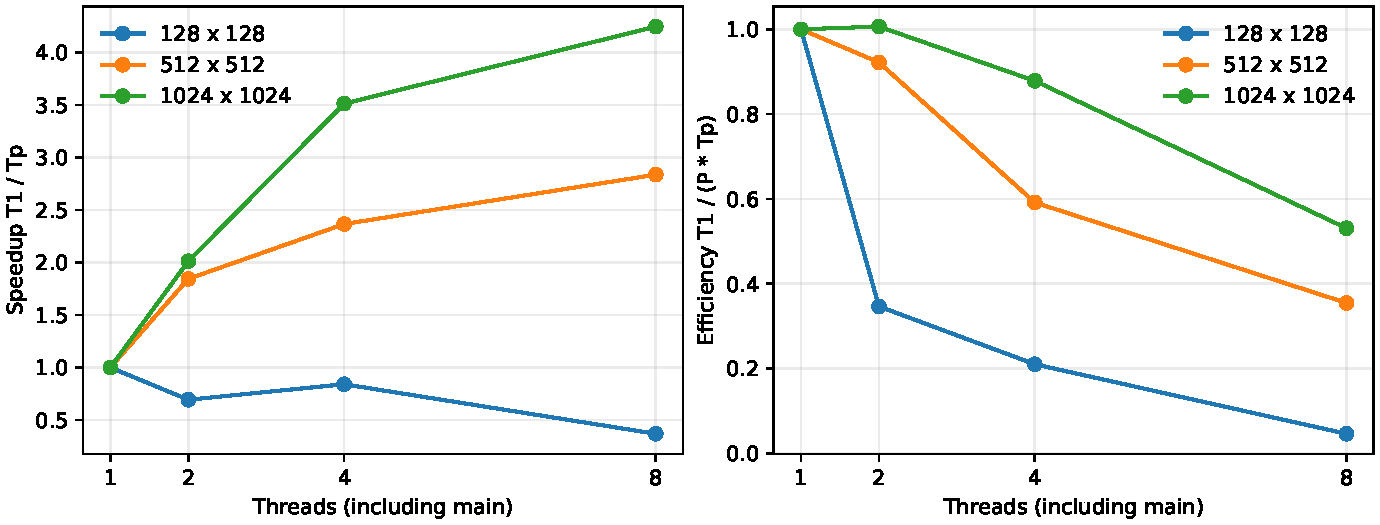
\includegraphics[width=\linewidth]{inc/scaling.pdf}
\caption{Ускорение и эффективность по медианам пяти повторов}
\end{figure}

Для 128 на 128 добавление потоков замедляет работу: объём вычислений недостаточен, чтобы компенсировать запуск работников и ожидание на каждом из 20 проходов. Для 512 на 512 и 1024 на 1024 рост объёма вычислений улучшает соотношение полезной работы и накладных расходов; восемь потоков дают ускорение примерно 2.84 и 4.25 соответственно.

Эффективность на восьми потоках составляет примерно 0.355 и 0.531 для двух больших размеров. Линейного ускорения нет: в измеренное время входят последовательные участки, распределение работы, создание потоков и ожидание наиболее медленного диапазона. Разброс может быть связан с планировщиком, конкуренцией за ресурсы и изменением частоты процессора; отдельные вклады этих причин не измерялись.

Для 1024 и P=2 получено $E_P\approx1.006$. Превышение единицы меньше одного процента и не доказывает сверхлинейное масштабирование: отношение медиан подвержено шуму измерений, что видно по диапазонам времени. Выводы относятся к этой машине, нагрузке и простому способу запуска потоков; универсальное ускорение не утверждается. Пилотные короткие запуски сохранены отдельно под префиксом pilot и в итоговой таблице не смешиваются с K=20.

\section{Проверки и независимое ревью}

Принудительная первоначальная сборка и последующие пересборки изменённых исходников прошли с указанными строгими флагами GCC. В tests/run.sh успешно выполнены 14 именованных групп проверок с дополнительными вариантами входов. Проверены единичное и асимметричное ядро, заранее известный ответ для сдвига, дробные и отрицательные значения, ядро больше матрицы, несколько проходов, неравные диапазоны строк, ограничение потоков, неверный и неполный ввод, субнормальные числа, переполнение вычислений и ошибка вывода.

Интерактивная проверка использует настоящий псевдотерминал и подтверждает повтор неверных строк. Отказы pthread\_create и pthread\_join проверяются отдельной сборкой с подменой этих функций через линкер. ASan и UBSan успешно выполнили те же 14 групп для основной программы; сценарии подмены pthread при этом используют отдельный обычный тестовый исполняемый файл. Санитайзеры не заменяют доказательство отсутствия гонок: оно основано на непересекающихся записях, неизменяемом входе и join перед сменой буферов.

Текстовые протоколы находятся в inc/checks.txt и inc/style.txt. Фактический вывод примера совпал с examples/expected.txt побайтово. Независимое ревью проверяет декомпозицию и владение ресурсами после реализации; заключение сохраняется в inc/review.txt. Проверка охватывает C11 и POSIX API, но не заявляет соответствия всем стандартам C++: язык задания -- C.

\section{Выводы}

Реализована многопоточная свёртка пользовательской матрицы с пользовательским ядром, K проходами и ограничением общего числа потоков ключом запуска. Синхронизация выполняется ожиданием завершения работников между проходами. Корректность подтверждена эталонными и граничными проверками, управление памятью -- дополнительными запусками с санитайзерами, число потоков -- наблюдениями ОС и трассой. Исследование показывает, что многопоточность полезна при достаточном объёме вычислений, но создаёт заметные накладные расходы на малых матрицах.

\appendixsection{А}{Исходный код}

\begin{listingblock}{Файл main.c}\inputcode{../src/main.c}\end{listingblock}

\begin{listingblock}{Файл matrix.h}\inputcode{../src/matrix.h}\end{listingblock}

\begin{listingblock}{Файл matrix.c}\inputcode{../src/matrix.c}\end{listingblock}

\begin{listingblock}{Файл filter.h}\inputcode{../src/filter.h}\end{listingblock}

\begin{listingblock}{Файл filter.c}\inputcode{../src/filter.c}\end{listingblock}

\begin{listingblock}{Файл console.h}\inputcode{../src/console.h}\end{listingblock}

\begin{listingblock}{Файл console.c}\inputcode{../src/console.c}\end{listingblock}

\end{document}
